Esta seção apresenta os procedimentos metodológicos adotados para o desenvolvimento e a avaliação da abordagem proposta. O método, ilustrado na Figura \ref{fig:method}, foi estruturado em três etapas principais: (i) materiais, (ii) pré-processamento e (iii) extração de características e treinamento dos modelos. Cada etapa é descrita detalhadamente nas seções subsequentes.

\begin{figure}[h]
    \centering
    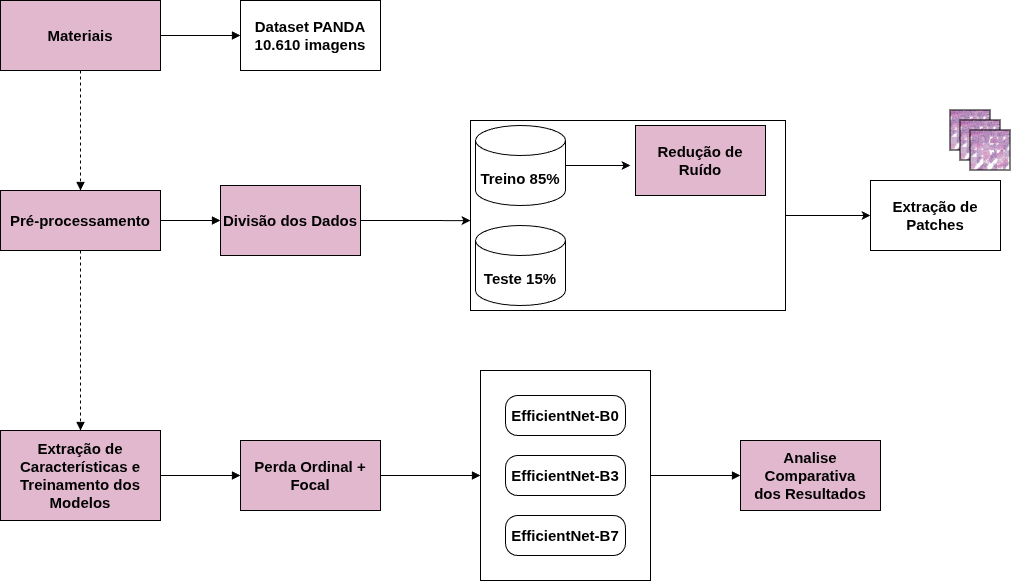
\includegraphics[width=0.9\linewidth]{images/method-semish.png}
    \caption{Método Proposto}
    \label{fig:method}
\end{figure}

\subsection{Materiais}
\label{sub:data}

Neste trabalho foi utilizada a base de dados PANDA (\textit{Prostate Cancer Grade Assessment}), composta por aproximadamente 10.616 imagens histopatológicas completas (\textit{Whole Slide Images} -- WSIs) de biópsias prostáticas \cite{ref-panda2020}. Esse conjunto de dados foi disponibilizado no contexto do desafio PANDA, promovido na plataforma Kaggle, e tem sido amplamente utilizado em pesquisas voltadas à classificação automática do câncer de próstata. As imagens presentes no banco de dados são anotadas com o escore e o grau de Gleason, fornecendo rótulos clínicos utilizados na graduação da doença. Neste estudo, foi utilizada exclusivamente a versão pública da base de dados, sem acesso ao conjunto privado disponibilizado durante o desafio.

Os dados foram coletados em dois centros médicos distintos, \textit{Radboud University Medical Center} e \textit{Karolinska Institute}, o que introduz variabilidade institucional nas imagens. Essa variabilidade está associada a diferenças nos protocolos de preparação das lâminas, digitalização e critérios de anotação, tornando o cenário experimental mais próximo da prática clínica real.

Além disso, o conjunto de dados apresenta ruídos inerentes ao processo de aquisição e anotação das lâminas. Entre eles, destacam-se artefatos visuais, como marcas de caneta realizadas por patologistas durante a análise das lâminas, conforme ilustrado na Figura~\ref{fig:pen_mask}. Também há ruídos relacionados à rotulação das imagens, como a discordância entre anotadores na atribuição dos graus histopatológicos. Esses fatores aumentam a complexidade da tarefa de classificação automática e refletem desafios presentes na prática da patologia digital.

\begin{figure}[htbp]
	\centering
	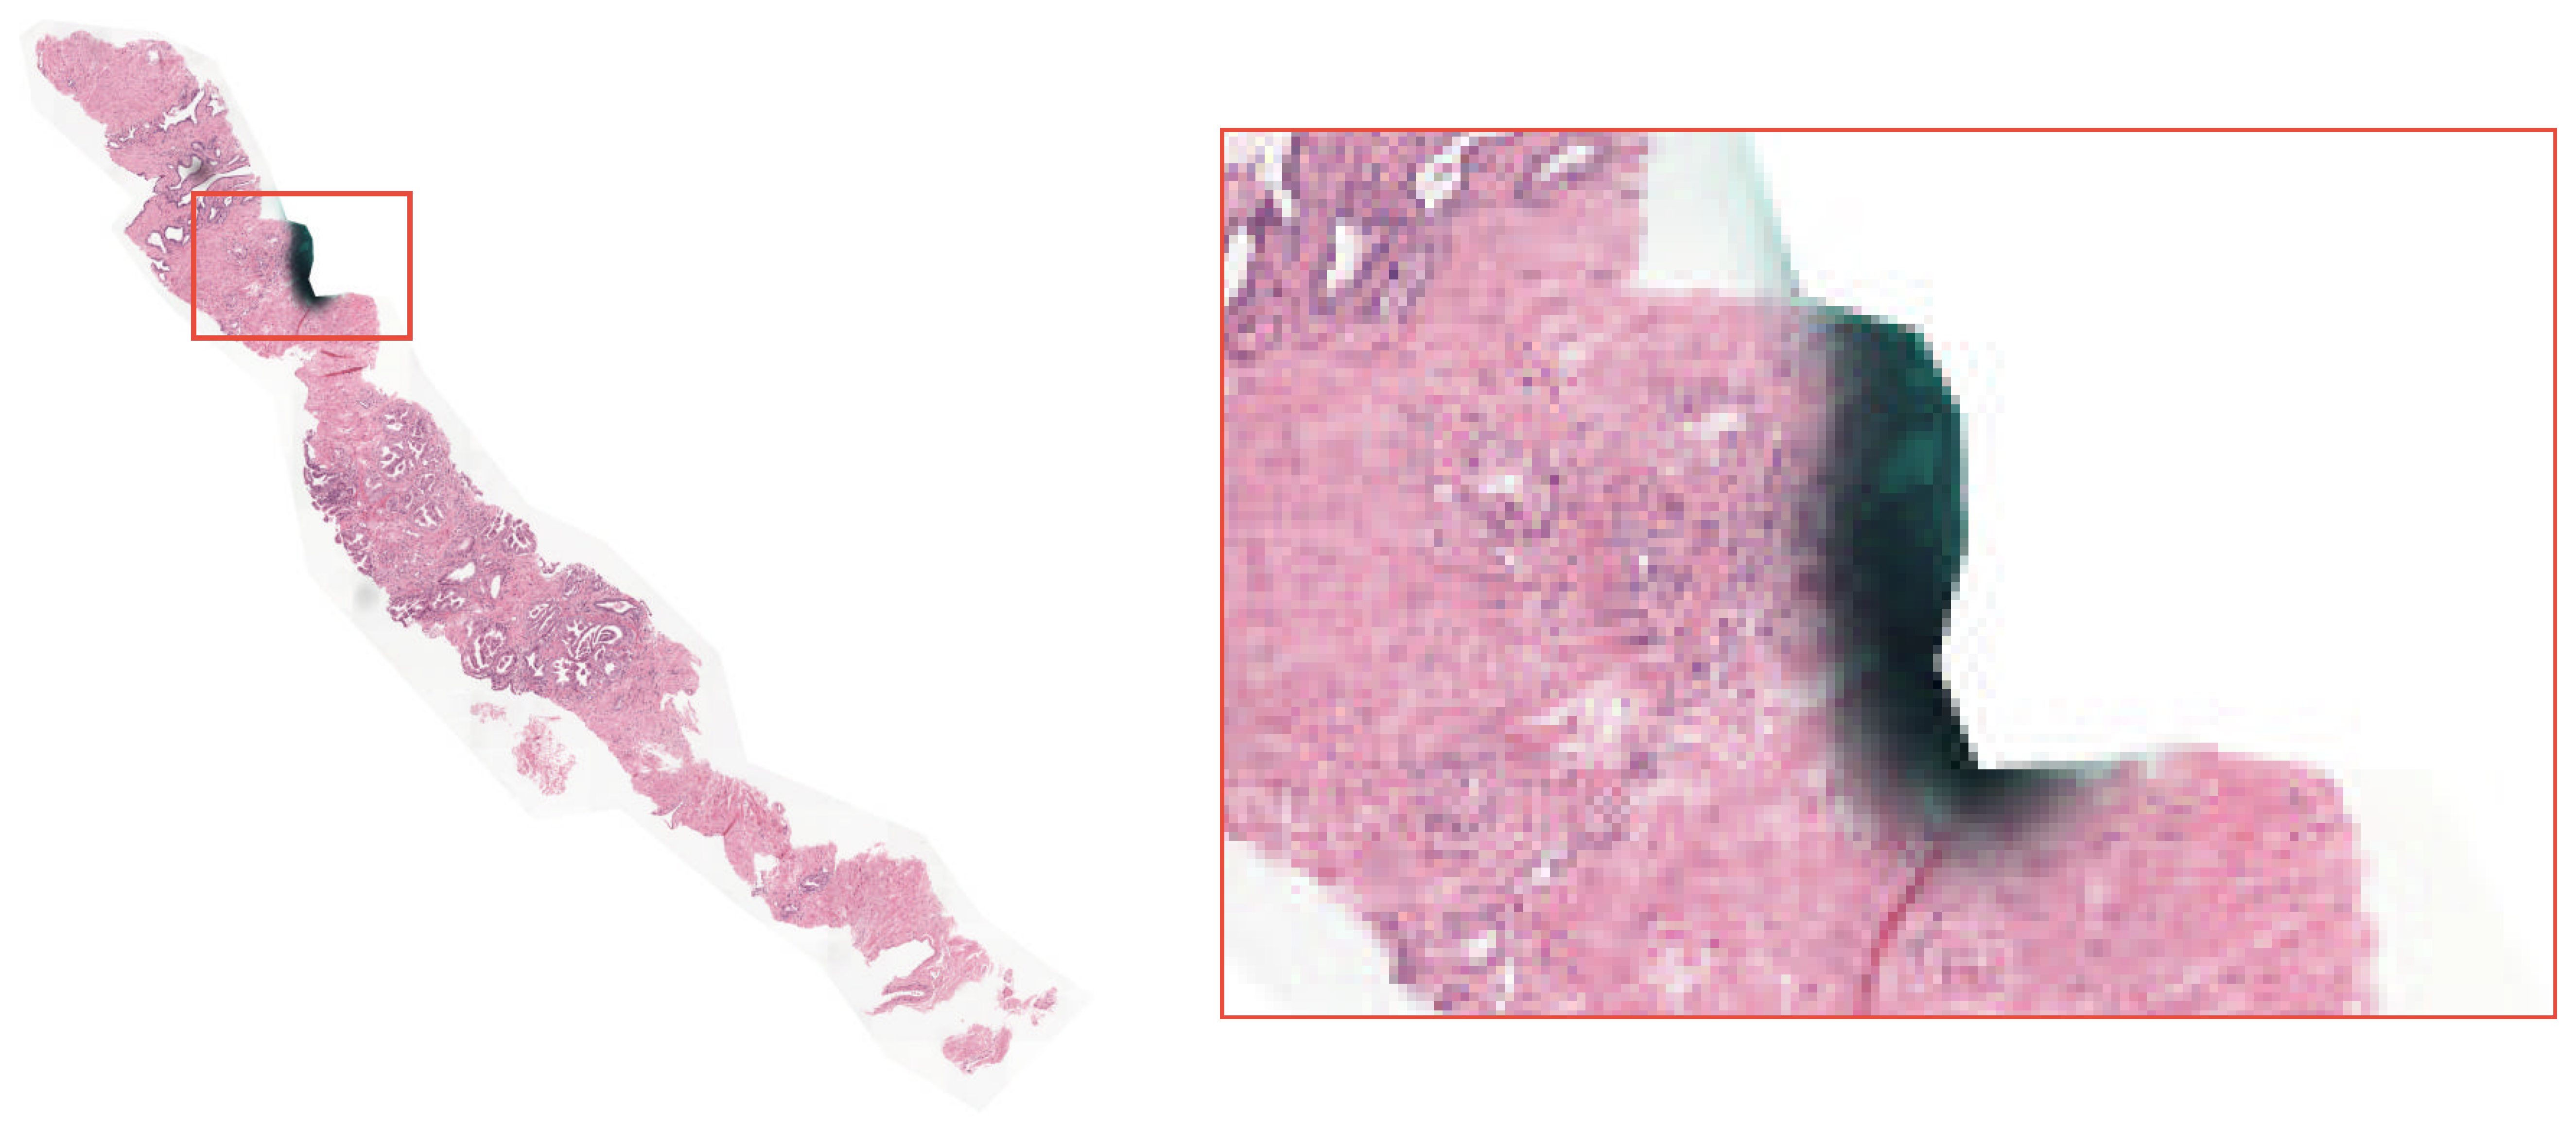
\includegraphics[width=0.8\linewidth]{images/zoom_region.png}
	\caption{Exemplo de artefato visual presente em uma WSI da base PANDA. À esquerda, apresenta-se a lâmina completa com a região de interesse destacada em vermelho. À direita, observa-se uma ampliação da região selecionada, evidenciando uma marca de caneta sobre o tecido prostático.}
	\label{fig:pen_mask}
\end{figure}

Outro aspecto relevante da base de dados é a distribuição desigual das amostras entre as seis classes de graduação ISUP (ISUP 0 a ISUP 5). Destaca-se que o grau ISUP 0 indica ausência de lesão maligna. Observa-se maior concentração de amostras nas classes ISUP 0 e ISUP 1, enquanto as demais apresentam menor representatividade. A distribuição completa das amostras é apresentada na Figura \ref{fig:distribuicao-isup}. %\ref{tab:distribuicao_panda}.

\begin{figure}[htb]
	\centering
	\includegraphics[width=1\textwidth,height=0.3\textheight]{"images/distribuição ISUP"}
	\caption{Distribuição das amostras da base PANDA}
	\label{fig:distribuicao-isup}	
\end{figure}


\subsection{Pré-processamento}
Na fase de pré-processamento, os dados foram inicialmente divididos em conjuntos de treinamento e teste, garantindo a separação adequada entre as etapas de ajuste e de avaliação do modelo. Em seguida, aplicou-se uma técnica de redução de ruído baseada em entropia e, por fim, realizou-se a extração de \textit{patches} a partir da densidade de informação de cada lâmina.

Para a etapa de redução de ruído, utilizaram-se quatro arquiteturas baseadas no \textit{backbone} EfficientNet (B0, B1, B2 e B3) para calcular a entropia de Shannon, a fim de quantificar a incerteza das predições \cite{ali2023entropy}. A entropia média dos quatro modelos foi calculada para cada amostra do conjunto de treinamento, e o percentil superior de 10\% foi selecionado, formando um banco de dados de amostras potencialmente ruidosas. A partir desse conjunto, avaliaram-se quatro cenários: manutenção integral dos dados e remoção de 100\%, 50\% e 20\% das imagens identificadas como ruidosas. O melhor desempenho foi obtido com a remoção de 20\% dessas imagens (180 amostras), indicando que muitas amostras, apesar de apresentarem alta incerteza, contribuem com informações relevantes para o problema no contexto do banco de dados.

Na etapa final do pré-processamento, a partir das WSIs do PANDA, foram geradas novas imagens por meio da extração de \textit{patches}, selecionando-se regiões de tecido relevante. Essa abordagem foi necessária porque o material histológico ocupa apenas parte da lâmina; sem a extração, o processamento direto das WSIs originais envolveria alto custo computacional e análise de grandes áreas sem tecido, como ilustrado na Figura~\ref{fig:original-panda}.

\begin{figure}[htb]
\centering

\includegraphics[width=0.8\linewidth]{images/original.png}
\caption{Exemplo de imagem do banco de dados PANDA}
\label{fig:original-panda}
\end{figure}

Para definir a melhor estratégia de extração, avaliou-se a reorganização das imagens em \textit{patches} nas configurações 5×5 (25 \textit{patches}), 6×6 (36 \textit{patches}) e 7×7 (49 \textit{patches}). Conforme ilustrado na Figura~\ref{fig:tiles-original}, a configuração 5×5 apresenta maior densidade de tecido e menor proporção de áreas vazias, mas o número reduzido de fragmentos pode levar à perda de regiões potencialmente relevantes, prejudicando a representação de padrões lesionais mais sutis. Por outro lado, a configuração 7×7 preserva maior cobertura espacial da lâmina, porém inclui muitas regiões sem tecido e gera imagens de alta dimensionalidade (1792×1792), o que aumenta a demanda por memória e tempo de processamento. Diante disso, optou-se pela configuração intermediária de 36 \textit{patches}, que preserva a maior parte da informação tecidual, mantendo a dimensionalidade relativamente reduzida (1536×1536), equilibrando qualidade, cobertura e eficiência computacional.
\begin{figure}[H]
	\centering
	
\includegraphics[width=0.9\textwidth]{images/tiles-original.png}
	%
	\caption{Ilustração da extração de \textit{patches} em diferentes tamanhos: 5x5 (à esquerda), 6x6 (no centro) e 7x7 (à direita).}
	\label{fig:tiles-original}%
\end{figure}

\subsection{Extração de características e treinamento dos modelos}

Nesta seção, apresenta-se a abordagem proposta para o treinamento dos classificadores individuais, incluindo a definição dos hiperparâmetros, das estratégias de regularização e da função de perda. Após o pré-processamento, iniciaram-se o treinamento e a avaliação dos classificadores. A EfficientNet-B0 foi utilizada como modelo-base para ajustar os hiperparâmetros. Com a configuração definida, os experimentos foram estendidos às EfficientNet-B3 e B7, permitindo comparar diferentes níveis de complexidade da mesma família e analisar o impacto da maior capacidade representacional no desempenho e na generalização.

Inicialmente, adotou-se a \textit{Binary Cross-Entropy} (BCE) como função de perda \textit{baseline}, em virtude de sua ampla utilização em cenários de classificação multirrótulo. A partir dessa configuração inicial, foram conduzidos experimentos exploratórios com o objetivo de analisar a estabilidade do treinamento e o impacto dos hiperparâmetros na capacidade de generalização do modelo. Foram avaliadas variações na taxa de aprendizado, no número de camadas descongeladas durante o \textit{fine-tuning} e nas estratégias de regularização por meio de \textit{Dropout}. Para a seleção da melhor combinação de hiperparâmetros, empregou-se uma busca sistemática em grade , aplicada ao modelo EfficientNet-B0. Essa busca foi realizada utilizando um subconjunto correspondente a 20\% do conjunto de treinamento, reservado para validação interna, permitindo a identificação da configuração com melhor desempenho antes do treinamento final.

Apesar da avaliação dessas configurações no treinamento, observou-se um desempenho estagnado que poderia estar associado não apenas à escolha dos hiperparâmetros, mas também à formulação da própria função de perda. Considerando que a graduação do câncer de próstata possui natureza ordinal, em que os erros entre classes adjacentes são menos severos do que entre classes mais distantes, o problema foi reformulado como uma regressão ordinal.

Nessa formulação, a predição do grau ISUP não é tratada como um problema multiclasse com categorias independentes, e sim como uma sequência de classificações binárias cumulativas. Para um grau ISUP $k \in \{0,\dots,5\}$, o rótulo é codificado como um vetor binário cumulativo, no qual os $k$ primeiros elementos assumem valor 1 e os demais, 0; por exemplo, o grau 3 é representado por $[1,1,1,0,0]$. A perda ordinal é então aplicada de forma independente a cada limiar do vetor, o que faz com que o erro total corresponda à soma das discrepâncias cumuladas. Essa modelagem impõe uma penalização proporcional à distância entre classes, de modo que erros mais distantes acarretam maior custo, preservando a estrutura hierárquica do problema.

Para mitigar o desbalanceamento dos dados (Seção \ref{sub:data}), a perda ordinal foi combinada à \textit{Focal Loss} \cite{lin2017focal, DINA2023100699, CHEN2026235}. Esta função modula a entropia cruzada para reduzir a influência de instâncias classificadas com alta confiança, priorizando amostras de maior incerteza diagnóstica. No presente estudo, configurou-se o fator de foco $\gamma = 2,0$ para atenuar a contribuição de exemplos fáceis e o peso $\alpha = 0,25$ para equilibrar a importância relativa entre as classes. Essa estratégia direciona a otimização para os casos mais complexos e sub-representados, fundamentais para a distinção precisa entre os graus ISUP.

\subsection{Métricas de avaliação}

Foram utilizadas as métricas de \textbf{acurácia} e de \textbf{$\kappa_{\text{quad}}$} (Kappa Quadrático Ponderado). A acurácia mensura a proporção de predições corretas em relação ao total de instâncias avaliadas \cite{baldi2000assessing}. Já o $\kappa_{\text{quad}}$ quantifica o grau de concordância entre as classes preditas e as reais, incorporando penalizações proporcionais à magnitude do erro, sendo especialmente adequado para problemas de natureza ordinal \cite{ref-cohen1968}. 

A variabilidade das métricas e os respectivos intervalos de confiança foram estimados por meio de bootstrap não paramétrico \cite{efron1979bootstrap}. A partir das predições do conjunto de teste, geraram-se 1.000 reamostragens com reposição, preservando-se a dimensão do conjunto original. Para cada iteração, recalcularam-se os indicadores de desempenho, permitindo derivar a média, o desvio padrão e o intervalo de confiança (IC) de 90\% através dos percentis 5\% e 95\%. Esta abordagem garante uma estimativa de incerteza robusta, prescindindo de pressupostos paramétricos sobre a distribuição dos dados.